\documentclass[a4paper,11pt]{article}
\usepackage[utf8]{inputenc}\usepackage[T1]{fontenc}
\usepackage[english]{babel}\usepackage{lmodern}\usepackage{microtype}
\usepackage{amsmath,amssymb}\usepackage{geometry}
\geometry{a4paper,left=2.2cm,right=2.2cm,top=2.0cm,bottom=2.0cm}
\usepackage{booktabs,array}\usepackage{xcolor}
\definecolor{bokug}{RGB}{0,135,60}\usepackage{tikz}
\usetikzlibrary{arrows.meta,calc}
\usepackage{fancyhdr}\pagestyle{fancy}
\renewcommand{\headrulewidth}{0.4pt}
\usepackage{enumitem}\setlength{\parindent}{0pt}\setlength{\parskip}{4pt}

\begin{document}
\fancyhead[L]{\small VU Mechanik – LAWI 100515 (PI)}\fancyhead[R]{\small SS 2026}\fancyfoot[C]{\thepage}
\begin{center}{\large\bfseries\color{bokug}University of Natural Resources and Life Sciences, Vienna (BOKU)}\\[2pt]{\large\bfseries VU Mechanik – LAWI 100515 (PI)}\\[4pt]Exam \textbf{Group A} \hfill Date: 26.06.2026\\[2pt]\rule{\linewidth}{0.4pt}\end{center}

\textbf{Given system}\par The planar system consists of bending beams and a truss connected by hinges.
\begin{center}
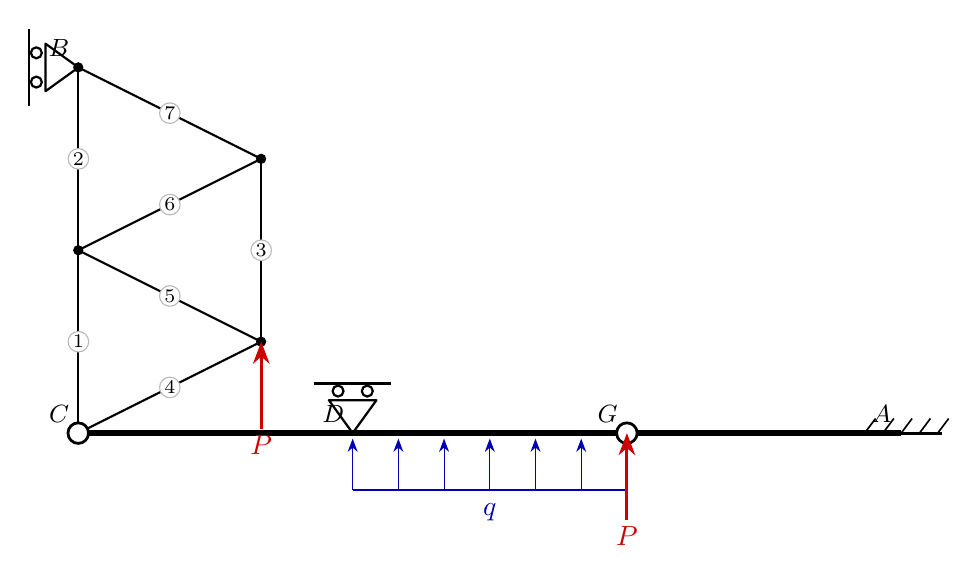
\begin{tikzpicture}[scale=1.161,>=Stealth,line join=round]
  \coordinate (P0) at (0.000,0.000);
  \coordinate (G) at (-3.000,0.000);
  \coordinate (D) at (-6.000,0.000);
  \coordinate (P1) at (-9.000,0.000);
  \coordinate (TO1) at (-9.000,2.000);
  \coordinate (TO2) at (-9.000,4.000);
  \coordinate (TU0) at (-7.000,1.000);
  \coordinate (TU1) at (-7.000,3.000);
  \draw[thick] (P1) -- (TO1);
  \draw[thick] (TO1) -- (TO2);
  \draw[thick] (TU0) -- (TU1);
  \draw[thick] (P1) -- (TU0);
  \draw[thick] (TU0) -- (TO1);
  \draw[thick] (TO1) -- (TU1);
  \draw[thick] (TU1) -- (TO2);
  \draw[line width=2.2pt] (P0) -- (G);
  \draw[line width=2.2pt] (G) -- (D);
  \draw[line width=2.2pt] (D) -- (P1);
  \fill (P1) circle (1.6pt);
  \fill (TO1) circle (1.6pt);
  \fill (TO2) circle (1.6pt);
  \fill (TU0) circle (1.6pt);
  \fill (TU1) circle (1.6pt);
  \draw[fill=white,line width=1pt] (P1) circle (3.2pt);
  \draw[fill=white,line width=1pt] (G) circle (3.2pt);
  \draw[line width=1.1pt] (0.450,0.000) -- (-0.450,0.000);
  \draw[line width=0.6pt] (0.400,0.000) -- (0.520,0.160);
  \draw[line width=0.6pt] (0.200,0.000) -- (0.320,0.160);
  \draw[line width=0.6pt] (0.000,0.000) -- (0.120,0.160);
  \draw[line width=0.6pt] (-0.200,0.000) -- (-0.080,0.160);
  \draw[line width=0.6pt] (-0.400,0.000) -- (-0.280,0.160);
  \draw[thick] (-6.000,0.000) -- (-5.740,0.360) -- (-6.260,0.360) -- cycle;
  \draw[thick] (-5.840,0.460) circle (0.06) (-6.160,0.460) circle (0.06);
  \draw[line width=1pt] (-5.580,0.540) -- (-6.420,0.540);
  \draw[thick] (-9.000,4.000) -- (-9.360,4.260) -- (-9.360,3.740) -- cycle;
  \draw[thick] (-9.460,4.160) circle (0.06) (-9.460,3.840) circle (0.06);
  \draw[line width=1pt] (-9.540,4.420) -- (-9.540,3.580);
  \node[circle,fill=white,draw=gray!55,inner sep=0.5pt,font=\scriptsize] at (-9.000,1.000) {1};
  \node[circle,fill=white,draw=gray!55,inner sep=0.5pt,font=\scriptsize] at (-9.000,3.000) {2};
  \node[circle,fill=white,draw=gray!55,inner sep=0.5pt,font=\scriptsize] at (-7.000,2.000) {3};
  \node[circle,fill=white,draw=gray!55,inner sep=0.5pt,font=\scriptsize] at (-8.000,0.500) {4};
  \node[circle,fill=white,draw=gray!55,inner sep=0.5pt,font=\scriptsize] at (-8.000,1.500) {5};
  \node[circle,fill=white,draw=gray!55,inner sep=0.5pt,font=\scriptsize] at (-8.000,2.500) {6};
  \node[circle,fill=white,draw=gray!55,inner sep=0.5pt,font=\scriptsize] at (-8.000,3.500) {7};
  \draw[->,blue!70!black] (-3.000,-0.620) -- (-3.000,-0.060);
  \draw[->,blue!70!black] (-3.500,-0.620) -- (-3.500,-0.060);
  \draw[->,blue!70!black] (-4.000,-0.620) -- (-4.000,-0.060);
  \draw[->,blue!70!black] (-4.500,-0.620) -- (-4.500,-0.060);
  \draw[->,blue!70!black] (-5.000,-0.620) -- (-5.000,-0.060);
  \draw[->,blue!70!black] (-5.500,-0.620) -- (-5.500,-0.060);
  \draw[->,blue!70!black] (-6.000,-0.620) -- (-6.000,-0.060);
  \draw[blue!70!black,thick] (-3.000,-0.620) -- (-6.000,-0.620);
  \node[blue!70!black] at (-4.500,-0.870) {$q$};
  \draw[->,red!80!black,line width=1.1pt] (-3.000,-0.950) -- (-3.000,0.000);
  \node[red!80!black] at (-3.000,-1.130) {$P$};
  \draw[->,red!80!black,line width=1.1pt] (-7.000,0.050) -- (-7.000,1.000);
  \node[red!80!black] at (-7.000,-0.130) {$P$};
  \node[font=\small] at (0.000,0.000) [xshift=-7pt,yshift=7pt] {$A$};
  \node[font=\small] at (-3.000,0.000) [xshift=-7pt,yshift=7pt] {$G$};
  \node[font=\small] at (-6.000,0.000) [xshift=-7pt,yshift=7pt] {$D$};
  \node[font=\small] at (-9.000,0.000) [xshift=-7pt,yshift=7pt] {$C$};
  \node[font=\small] at (-9.000,4.000) [xshift=-7pt,yshift=7pt] {$B$};
\end{tikzpicture}
\end{center}
\textbf{Given quantities:}\quad $a=3$\,m\quad $\ell=2$\,m\quad $h=2$\,m\quad $q=5$\,kN/m\quad $P=20$\,kN
\par\medskip
\textbf{Tasks}\par
\begin{enumerate}[label=\textbf{\arabic*.}]
  \item Determine the degree of static determinacy.
  \item Compute all support reactions and hinge forces.
  \item Determine all truss member forces (tension/compression).
  \item Draw the section forces $N$, $V$, $M$ of the bending beams.
\end{enumerate}
\end{document}